\section{Automatic Detection in Magnetostatic Surveys using Convolutional Neural Networks}
I started work in the field of automated detection in geophysical surveys in 2017, where I first developed, with the help of my colleague Fabien GOGLIO, a simple \gls{cnn} that could categorise low resolution images of magnetostatic surveys. 

The aim of this project was to be able to detect two type of classes of features: "Anomalies" and "Object"

\begin{itemize}
	\item The ”Anomaly” Class, contemporary ferromagnetic objects : small, localized, point-like disturbance, possessing both a global maxima situated at the center and global minima around the center, in the shape of a halo. They are usually cause by a metallic artefact. 
	\item The ”Object” Class, anthropogenic activity : a linear shape which is not localized at a particular point, and can form more complex geometric shape, such as rectangles. Objects can also be found in non linear forms. They possess smoother gradients variations, and are in general bigger than anomalies. Their intensity is often not consistent, creating ”blobs”.
\end{itemize}

\begin{figure}[ht]
	\begin{subfigure}{.5\textwidth}
		\centering
		% include first image
		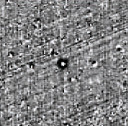
\includegraphics[width=.8\linewidth]{AnomalieEx}  
		\caption{Anomaly}
		\label{fig:anomalyEx}
	\end{subfigure}
	\begin{subfigure}{.5\textwidth}
		\centering
		% include second image
		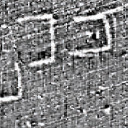
\includegraphics[width=.8\linewidth]{FeatureEx}  
		\caption{Object}
		\label{fig:anomalyExample}
	\end{subfigure}
	\caption{Examples of Anomaly and Object class. Detail from a survey done in Bergères Les Vertues, Eastern France}
	\label{fig:exClasses}
\end{figure}

\subsection{Dataset}
Those surveys were centered mainly on the archaeological dig of Marsal, France, along with various other small scales surveys done around the UK. The project proved to be a success, with high precision being achieved rapidly. However, this was just a proof of concept; showcasing that this kind of techniques could work for this type of data which is very challenging for traditional computer vision. 


From those surveys, a 2 new datasets were created, one for classification using \glspl{cnn}, and another for use with the \gls{yolo} model. 

The first dataset was constructed by first manually selecting zones containing at least one example of a class, and then segmenting those zones into $128 \times 128$ tiles, with an overlap of 48 pixels. Some typical data augmentation was added to make the dataset more robust, like random flipping and rotations. 

The second dataset used larger regions of about $1000 \times 1000$ pixels, which were annotated using LabelImg\cite{labelImg}. The full sized images were not used as it would result in a massive loss of detail when \gls{yolo} would downscale it.  

\subsection{Models}
The first model used a low input resolution $128\times 128$ pixel square segmented from the image itself to predict whether the image contained an ``anomaly' or an archaeological feature. The model was a simple \gls{cnn} with a 8 layers of 2D convolution, with 2 layers of Fully Connected to output a $2 \times 1$ vector.  

The second model used YOLOv3-tiny\cite{yolov3}, a novel technique at the time to detect the same classes of objects. The YOLO architecture was not modified, but it was noticed that the tiny version of the YOLO architecture, designed to run on low power computers performed better than the large version. 

\subsection{Results}
The CNN performance was very good, with over 90\% accuracy on the validation dataset.

Results for the YOLO model were encouraging, with class prediction precision at around 95\% and an average IoU havering around 55\%. However, the reduced size of the dataset massively impacted the F1-Score, coming out at only 0.16.

\section{Learning To Look At LiDAR}\label{learningLidar}
This paper, authored by Verschoof-van der Vaart and Lambers\cite{wouter2019}, proposes the use of Deep Learning models for automated object detection using Faster-RCNN\cite{FasterRCNN} on \gls{lidar} surveys. It presents a novel dataset based on \gls{lidar} surveys of a large and archaeologically rich region of the Netherlands, along with a framework for detection of 3 classes of objects based on Faster-RCNN.

\subsection{Dataset and WODAN}
The dataset used is novel, and part of the research effort was to create a workflow that would enable precise annotation of it. \gls{lidar} surveys were taken from a large central area in the Netherlands, know as the \textit{Utrechtse Heuvelug} and the \textit{Veluwe} This area is largely forested and is about $\sim 2350 \text{km}^2$ in size. 


The dataset was mostly constructed by hand, with human verifications of each image. Using LabelImg\cite{labelImg}, the authors annotated each TIF images. In total, the dataset is comprised of 420 images, split into three sub dataset: 365 images were used for training, 41 for validation and 73 for testing. Some data augmentations in the form of horizontal and vertical flips, along with 90 degrees rotations. 

\subsection{Model}
The model used here is an altered version of Faster-RCNN with a validation step added after every two epochs to check for possible \gls{overfit}.
The model was trained over 12-18 epochs because of the small dataset, using pretrained weights.

Experiments were done using two different backbone: ResNet50\cite{resNet} and VGG16\cite{vgg}. Those experiments aimed to measure the impact a change in the stride of the \gls{rpn} and the anchors size had on performance. 

\subsection{Results}

\begin{table}[h]
	\centering
	\begin{tabular}{lllllll}
		Experiment & Epochs & Anchorsboxes & Recall    & Precision & F1        & MaF1 \\\midrule
		1          & 12     & 16, 64, 512  & 0.76/0.19 & 0.57/0.71 & 0.65/0.30 & 0.43 \\
		2          & 15     & 16, 64, 128  & 0.78/0.48 & 0.36/0.47 & 0.49/0.47 & 0.47 \\
		3          & 15     & 16, 64, 256  & 0.69/0.97 & 0.77/0.26 & 0.73/0.41 & 0.45 \\
		4          & 15     & 16, 64, 384  & 0.71/0.92 & 0.90/0.26 & 0.79/0.41 & 0.46 \\
		5          & 15     & 16, 64, 512  & 0.62/0.82 & 0.55/0.58 & 0.59/0.68 & 0.66 \\
		6          & 18     & 16, 64, 512  & 0.81/0.20 & 0.68/0.50 & 0.74/0.29 & 0.44 \\\bottomrule
	\end{tabular}
	\caption{Results of the experiments. Values before slash are for barrows, after slash are for Celtic Fields.}
	\label{tab:learningLidarRes}
\end{table}

The results of the different experiments are reproduced in Table~\ref{tab:learningLidarRes}. Those experiments were done using the VGG16 backbone. The average of precision of Celtic Field detections is 0.46, and recall is 0.60. Barrows fare better with average precision at 0.64 and recall at 0.73.

During all experiments, Faster R-CNN failed to detect charcoal kilns, probably due to the low quantity of examples in the dataset. 

\section{Integrating Remote Sensing, Machine Learning, and Citizen Science in Dutch Archaeological Prospection}\label{heritageQuest}

This article by Lambers, Verschoof-van der Vaart and Bourgeois\cite{lamberVerschoof2019} presents novel methods for multi class object detection in \gls{lidar} using Deep Learning combined with a citizen science project. 


\subsection{Dataset and Citizen Science}
The dataset is comprised of more than 430 $km^2$ of interpolated \gls{lidar} data gathered from the \textit{Veluwe} region. The image in the dataset have previously been used in another paper by Verschoof-van der Vaart and Lambers \cite{wouter2019} and are described in section \ref{learningLidar}. This paper presents a novel workflow to annotate the dataset, which is based on Citizen Science. 

This workflow stems from the issue of the lack of a large dataset labelled with Archaeological objects, and the presence of unknown Archaeological objects that have to be validated. Since such a dataset didn't exist at the time of creation of WODAN, it had to be created. 

Citizen Science is the use of volunteers and non professional scientists. Those citizen researchers helps with a scientific inquiry. In this project, a workflow based on Citizen Science generates datasets used for machine learning models and to validate new potential archaeological objects. Figure \ref{wodanApproach} shows the workflow used.

\begin{figure}[H]
  \centering
	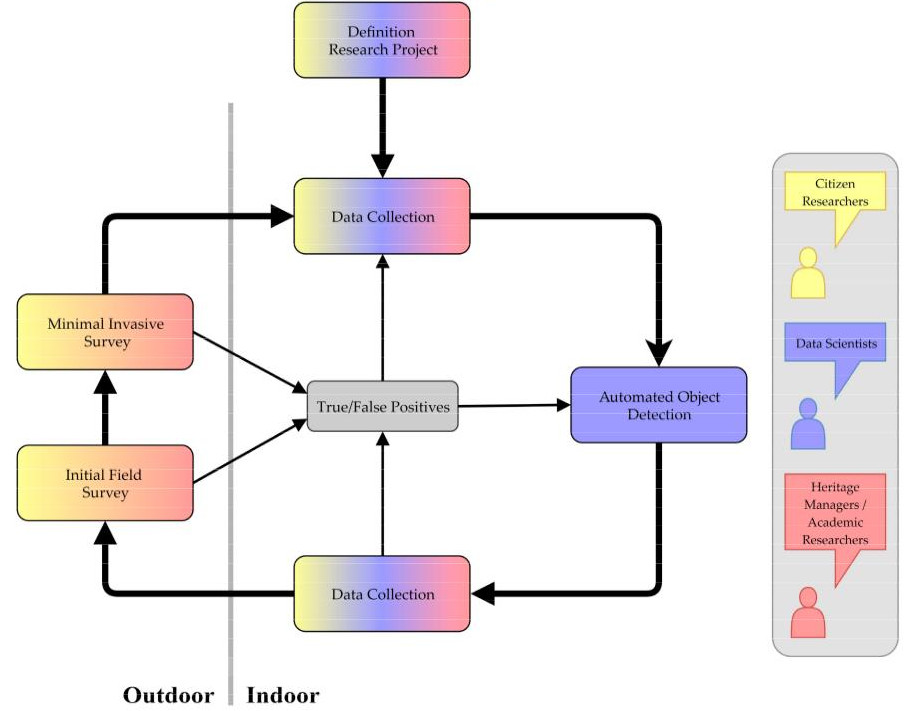
\includegraphics[width=0.8\textwidth]{wodan.jpg}
	\caption[]{Proposed workflow. The color indicates the different interest groups}
  \label{wodanApproach}
\end{figure}

\subsection{Validation}
After the data collection and automated object detection , the new potential archaeological objects are validated in three steps, following the Dutch research strategy: desktop survey, initial field survey and minimally invasive survey. Theses steps conducted by different groups of citizen researchers in collaboration with academic researchers. 

The desktop survey serves as a first validation steps, where the results of the prior steps, especially automated object detection will be verified for quality. The results are compared with digital informations sources, like aerial photographs and other remotely sensed data. This first steps allows for the detection of false positives and might lead to new archaeological insights.

The initial field survey serves as the first real verification step in the field, where newly discovered potential archaeological objects will be investigated. A predefined sets of characteristics such as dimensions, height, position etc. This validation steps also serves to detect false positives and might lead to the recognition of important parameters of archaeological objects. 

The final verification steps involve direct investigation potential archaeological object with minimally invasive techniques, like hand corings or test trench.  

The validations steps serves to determine true and false positives in detection, parameters of the archaeological objects and identification of new data sources. These results are then used to update the data collection and automated object detection. 

\subsection{Implementation}
The \gls{lidar} data is being analyzed using the Zooniverse, a website offering citizen science projects. In this project, baptised Heritage Quest, participants are asked to annotate every potential barrow, Celtic field or charcoal kiln in a given \gls{lidar} image. The user can switch between two \gls{lidar} representation, either shaded relief or Simple Local Relief Model. Each \gls{lidar} image will be classified by at least 8 different users, to minimize the inter-analyst variability. 

\section{Combining Deep Learning and Location-Based Ranking for Large-Scale Archaeological Prospection of LiDAR Data from The Netherlands}
This paper presents a more advanced version of WODAN, named simply WODAN2.0, a workflow using Deep Learning for automated detection of archaeological objects in \gls{lidar} data. WODAN2.0 adds a step of Location Based Ranking to reduce the false positive rate based on location in the detection workflow. 

\subsection{Dataset}
The dataset used used here is based on the same \gls{lidar} survey as Section \ref{learningLidar}, or WODAN1.0. 16 Tiles of \gls{lidar} data were used, each measuring $10000 \times 12500$ pixels or 5km $\times$ 6.25km. Those tiles were then cut into subtiles measuring $600 \times 600$ with 30 pixels overlap on all sides. Subtiles containing archaeological objects were selected and labeled with LabelImg. The final dataset contained 1024 subtiles for the training subset and 88 subtiles for the validation subset. 

WODAN1.0 only included distinct examples of archaeological objects, WODAN2.0 also includes less clearly visible examples of object. 

Negative Examples, or subtiles without any examples were also added as an experiment. Negative Examples can help the model learn background texture features, and potentially reduce the number of false positives.

\subsection{Model and Training}
The model used here is a modified FasterRCNN\cite{FasterRCNN}. 

\subsection{Location Based Ranking}
To make WODAN2.0 more robust and precise over different types of terrain, domain information needed to be introduced to the classification to reduce the number of false positives. \gls{lbr} was introduced as a step in the detection workflow. \gls{lbr} is based on the assumption that the location of archaeological objects is not entirely random but based on certain characteristics of past and present environment. 

\gls{lbr} consists of determining, ranking and mapping the principal landscape characteristics, like subsoil and land-use that have had an impact on the preservation of archaeological objects. \gls{lbr} produces a ranked map on which the location of detection can be compared and assigned to different ranks. Detections in high ranking zones are more likely to be archaeological objects, while detections in low ranking zones are more likely to be false positives. 
\subsection{Results}
Table \ref{tab:resWODAN2} shows the results of WODAN1.0 and WODAN2.0 against Heritage Quest, the Citizen Science project aiming at annotating the \gls{lidar} surveys and presented in section \gls{heritageQuest}. While WODAN obtain better performance on certain metrics, it is still inferior to human detection. 
\begin{table}[H]
	\centering
	\begin{tabular}{llllllllll}
		\hline
		Method             & \multicolumn{3}{c}{Kilns}                     & \multicolumn{3}{l}{Celtic Fields}         & \multicolumn{3}{l}{Charcoal Kilns}            \\ \hline
		                   & Recall        & Precision     & F1            & Recall        & Precision & F1            & Recall        & Precision     & F1            \\ \hline
				   WODAN1.0 (NR)      & \textbf{62.3} & 55.2          & 58.5          & \textbf{82.3} & 57.66     & 57.8          & -             & -             & -             \\
				   WODAN1.0 (R)       & 53.3          & 9.0           & 15.3          & 43.0          & 20.5      & 27.7          & -             & -             & -             \\ \hline
				   WODAN2.0 (NR)      & 57.1          & 73.3          & \textbf{70.1} & 74.6          & 66.0      & 70.0          & -             & -             & -             \\
				   WODAN2.0 (R)      & 44.5          & 56.5          & 49.8          & 40.4          & 52.1      & 45.5          & 34.6          & 12.2          & 18.0          \\
				   WODAN2.0+NEG (R)      & 47.4          & 46.4          & 46.9          & 38.5          & 45.4      & 41.7          & 19.2          & 10.2          & 13.3          \\ \hline
				   Heritage Quest (R) & 45.3          & \textbf{80.5} & 57.9          & 75.7          & 85.0      & \textbf{80.1} & \textbf{38.5} & \textbf{55.6} & \textbf{45.5}
	\end{tabular}
	\caption{Performance of WODAN1.0, WODAN2.0 and Heritage Quest on individual class. Non Random (NR) and Random (R) dataset are shown, NEG indicates the use of negative examples. Bold indicates best result.}
	\label{tab:resWODAN2}
\end{table}
